\Introduction

Галактики не расположены случайным образом в пространстве. Они формируют собой особые структуры, 
такие как скопления и сверхскопления галактик. Скопления в свою очередь часто представляют собой цепи, 
или так называемые "нити", на пересечении которых оказываются скопления галактик.\\

\begin{figure}
    \center{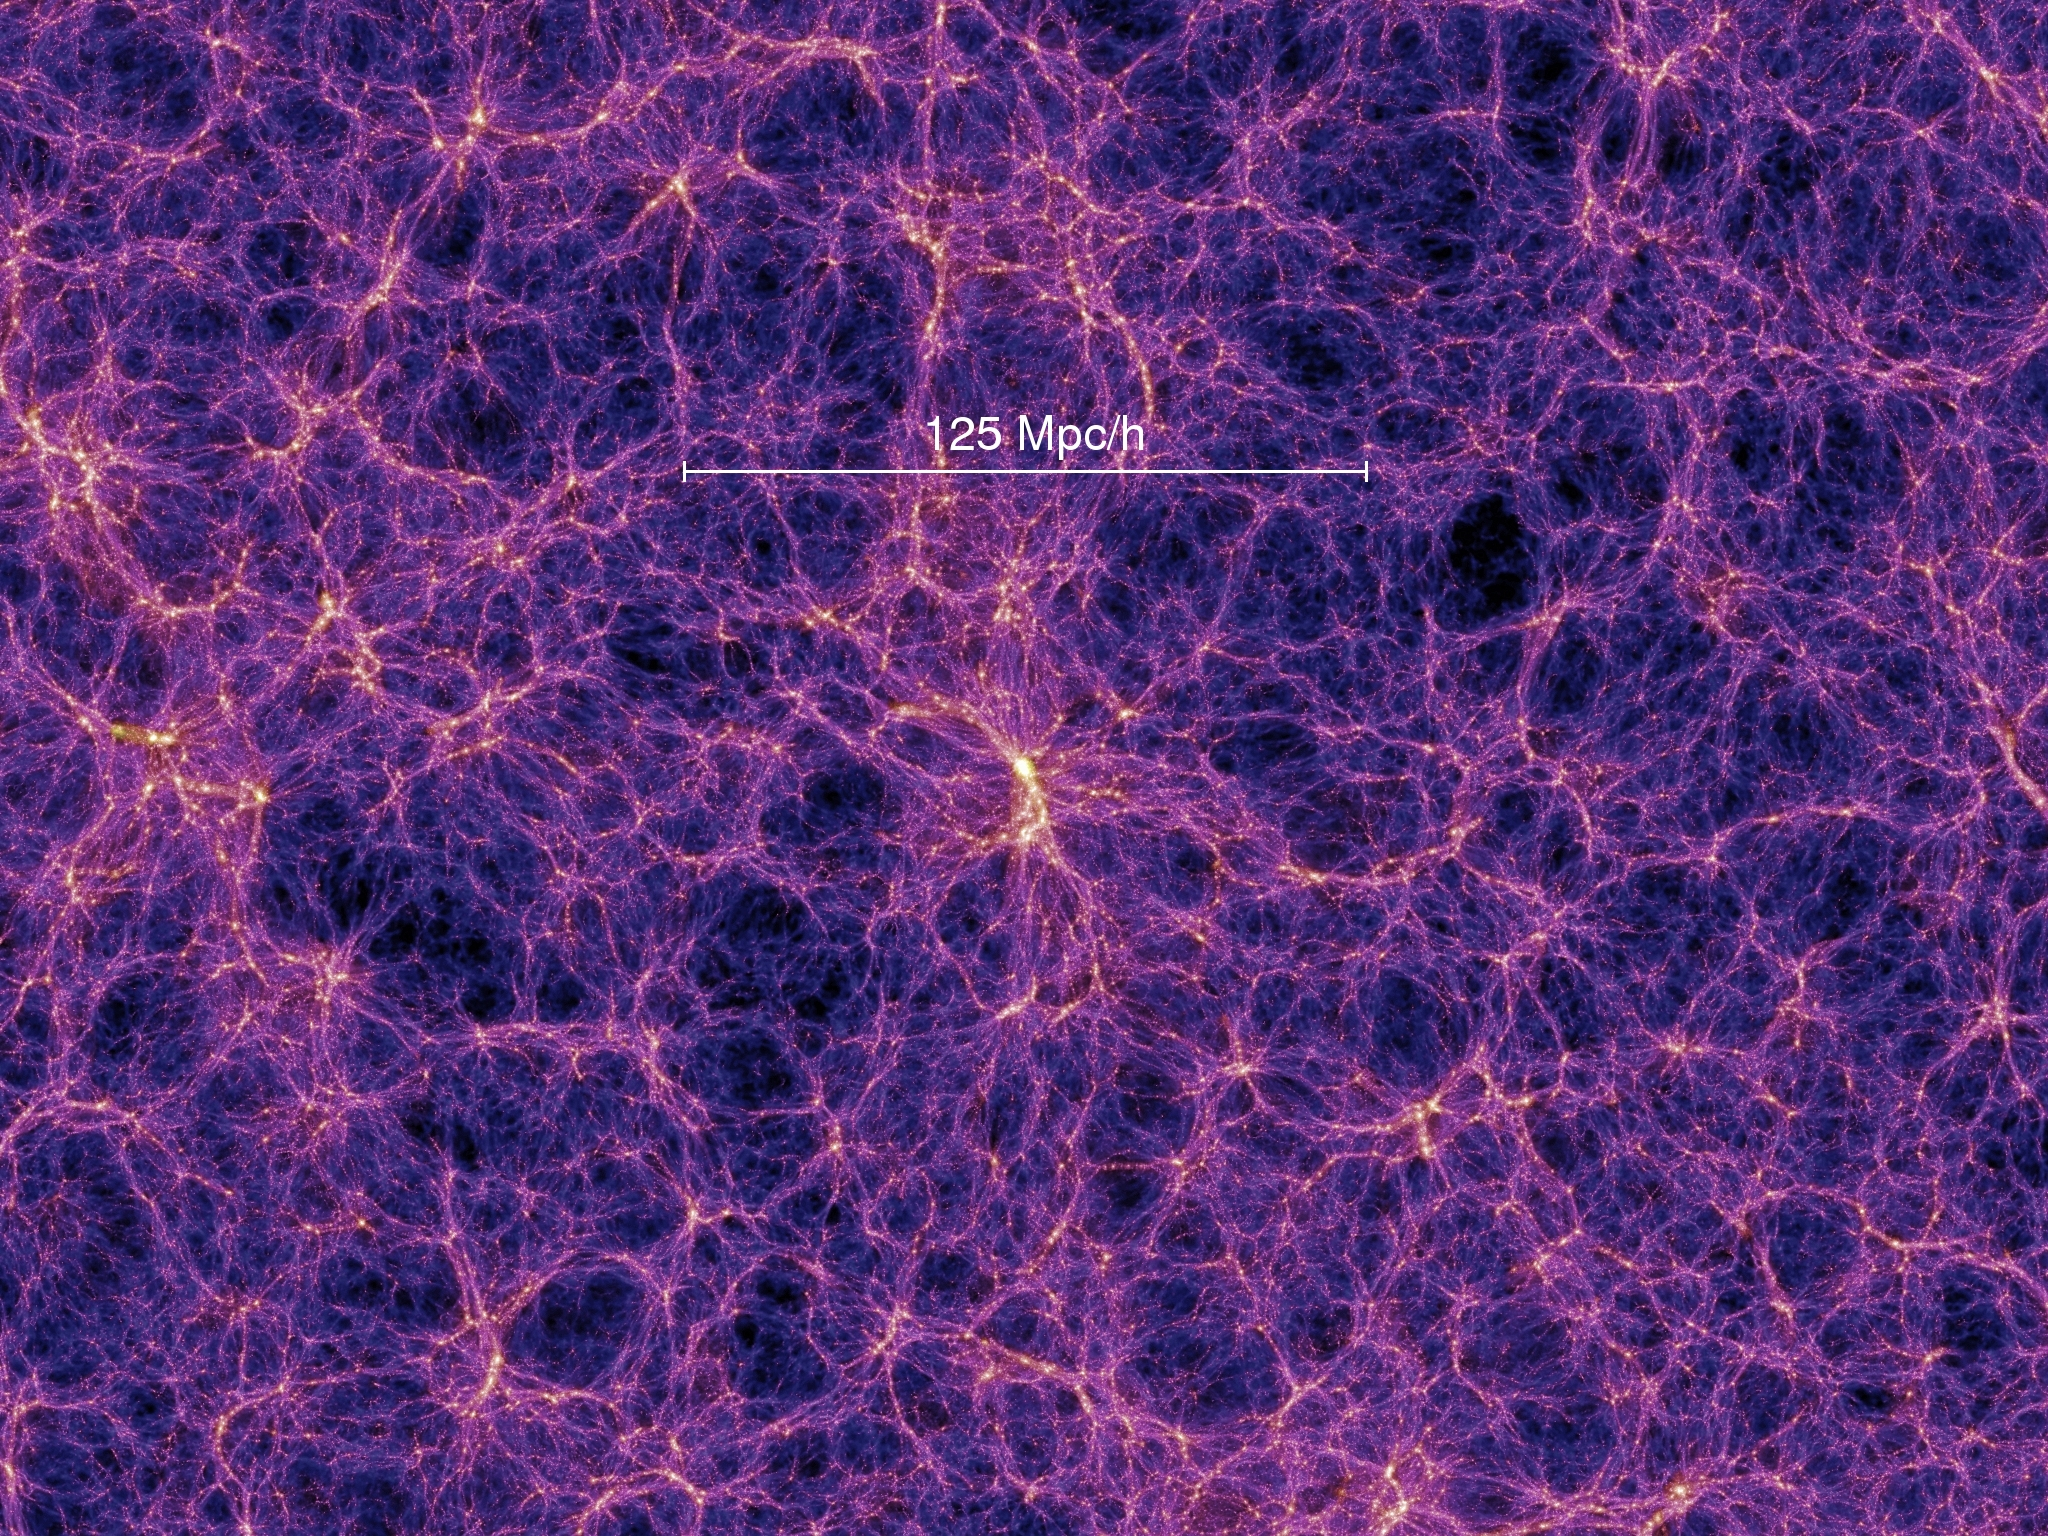
\includegraphics[width=0.6\linewidth]{model}}
    \caption{Моделирование «Милленниум» — N-частичное моделирование, проведённое Консорциумом 
        Девы с целью изучения формирования крупномасштабной структуры Вселенной в стандартной
        космологической модели.}
\end{figure}

Скопления галактик представляют большой интерес для исследования, так как их свойства сильно зависят 
от космологических параметров. Изучая их свойства, можно делать выводы о структуре обозримой части 
Вселенной. По большей части скопления состоят из тёмной материи, свойства которой до сих пор не 
известны науке. Поэтому через историю развития скоплений галактик можно изучать тёмную материю.\\

Сама по себе крупномасштабная структура Вселенной имеет объяснение. Через какое-то время после 
появления Вселенной возмущения волн плотности средних и больших масштабов при совпадении пиков 
образовали сверхскопления, в то время как сопадения фаз низкой плотности образовали войды - 
огромные пространства между нитями скоплений, в которых почти отсутствуют галактики и скопления. 
Таким образом, зная расположение и параметры большого количества скоплений, можно сделать выводы о 
том, как развивалась Вселенная на поздних этапах. \cite{Planck}\\

Одним из первых каталогов скоплений стал каталог Abell \cite{Abell}. Этот каталог содержит $4073$ 
богатых скопления галактик с красными смещениями $z < 0.2$. Он был построен при исользовании 
оптических данных обзора NGS-POSS.\\

\begin{figure}
    \center{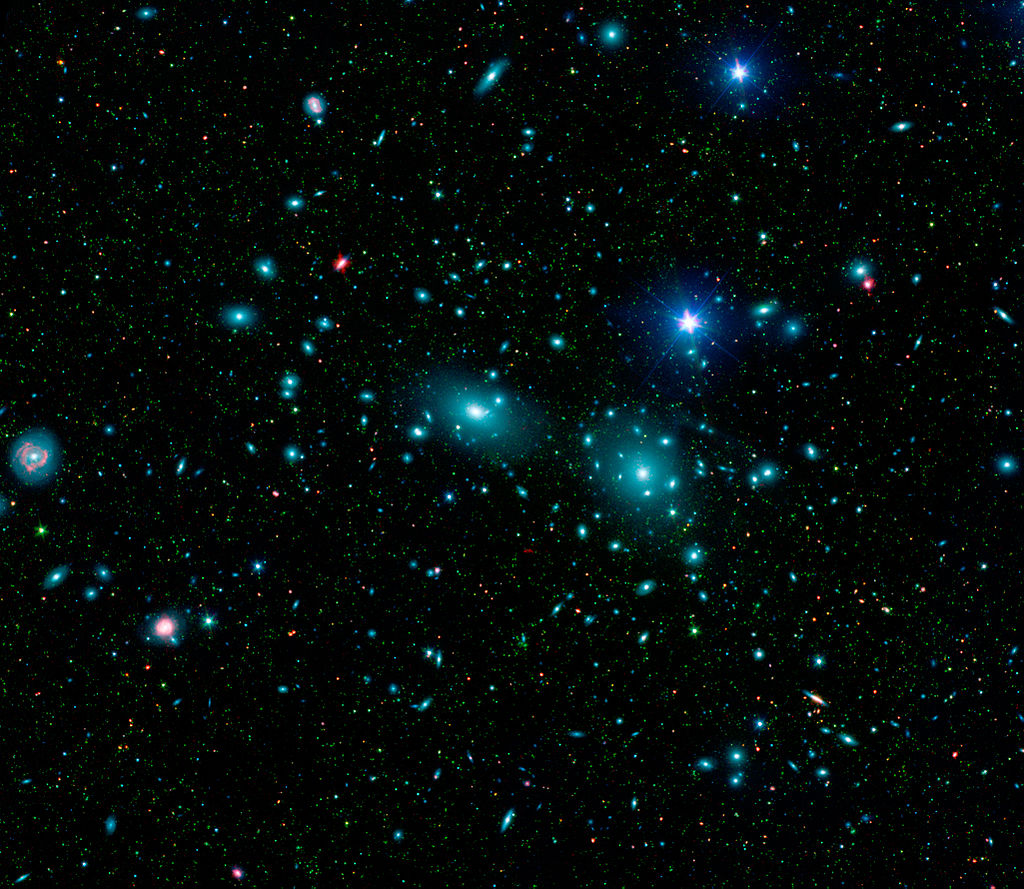
\includegraphics[width=0.6\linewidth]{coma_sdss}}
    \caption{Скопление Волос Вероники (Abell 1656) в обзоре SDSS - одно из самых известных 
        скоплений каталога Abell}
\end{figure}

Позднее были созданы каталоги с использованием других диапазонов. Далее для исследования будут 
использоваться следующие каталоги:\\

\begin{itemize}
\item PSZ2 - каталог, основанный на данных микроволнового обзора Planck. Был создан при 
    использовании алгоритмов Matched Multi-Filter и PowellSnakes.\\

\item MCXC - компиляция разных каталогов скоплений, все из которых основаны на данных рахных
    рентгеновских обзоров.\\

\item RedMaPPer - каталог, основанный на данных оптического обзора SDSS. Был создан при помощи 
    одноимённого алгоритма.\\

\item ACT - каталог, основанный на данных микроволнового обзора ACT. Был создан при помощи 
    алгоритма Matched Multi-Filter.\\
\end{itemize}

Создание каталогов данных в других диапазонах может помочь уточнить данные рентгеновских каталогов,
созданных классическими алгоритмами.\\

Кроме того, сама задача применения нейросетевых методов к детекции скоплений актуальна, так как 
методы глубокого обучения дают следующие преимущества при анализе данных:\\
\begin{itemize}
    \item Стандартные алгоритмы сегментации усредняют информацию по нескольким каналам, в то время 
        как с помощью нейросети можно охватить данные полностью.\\ 
    \item Каждый из классических методов имеет свои достоинства и недостатки, и для каждого 
        диапазона излучения существуют свои алгоритмы, в то время как нейросеть может стать 
        универсальным средством для сегментации данных нескольких каналов одновременно.\\
\end{itemize}


